% IEEE conference paper (max 4 pages) based on IEEEtran bare_conf template.
\documentclass[conference]{IEEEtran}

% Basic packages (keep minimal for page limit)
\usepackage[utf8]{inputenc}
\usepackage{graphicx}
\usepackage{amsmath}
\usepackage{booktabs} 
\usepackage{siunitx}
\usepackage{cite}
\usepackage[section]{placeins}
\usepackage{tikz}
\usetikzlibrary{arrows.meta}
\usetikzlibrary{positioning,arrows.meta}

% Ensure figures stay in column width
\setlength{\textfloatsep}{8pt}
\setlength{\floatsep}{8pt}
\setlength{\intextsep}{8pt}

% Clickable references with hidden link styling.
\usepackage[hidelinks]{hyperref}

\begin{document}

\title{Evaluating Multimodal Alignment in ChatGPT and
Gemini: An Empirical Study of Inter- and
Intra-Model Consistency in Image Description and
Generation}

\author{\IEEEauthorblockN{Saverio Napolitano}
\IEEEauthorblockA{Mid Sweden University\\
sana2504@student.miun.se}}
   
\maketitle 

\begin{abstract}
This small, controlled study examines how well three perceptual metrics---LPIPS, CLIP cosine similarity, and MS-SSIM---align with human preferences over image variants generated by ChatGPT (DALL--E) and Gemini for 15 reference images. Ten raters ranked four variants per reference image. Inter-rater agreement (Kendall's W) is computed, automatic scores are summarized, and the correlation between human mean ranks and each automatic metric is measured. Humans show moderate agreement ($\bar{W}=0.40$). Across variants, automatic metrics favor different candidates, and only CLIP shows a modest positive correlation with human ranks on this dataset (mean Spearman $0.36$). LPIPS and MS-SSIM correlate weakly. These findings suggest that single off-the-shelf metrics are insufficient proxies for human judgments on this task and that model selection should incorporate targeted human feedback.
\end{abstract}

\begin{IEEEkeywords}
human evaluation, perceptual metrics, LPIPS, CLIP, MS-SSIM, alignment
\end{IEEEkeywords}
 
\section{Introduction}
Text-to-image systems are typically benchmarked with automatic similarity scores, yet deployment decisions rely on human perception. This study investigates how three widely used metrics align with human preferences over 15 sets of four image variants each. The main contribution is to show, in a small but controlled setting, how three popular metrics diverge from human rankings in a realistic 4-candidate selection scenario, and to quantify intra- vs inter-model consistency for ChatGPT and Gemini.

Two research questions structure the study:
\begin{enumerate}
    \item[RQ1] How consistent, with respect to human preferences, are ChatGPT and Gemini in aligning descriptions and generations, both within the same model and across different models?
    \item[RQ2] How well do LPIPS, MS-SSIM, and CLIP cosine similarity align with human judgments?
\end{enumerate}

Few studies contrast multiple perceptual metrics against ground-truth human orderings for images. By keeping the study small and controlled (15 reference images, fixed four-way choice), the behavior of off-the-shelf metrics is isolated without confounds from model sampling stochasticity. Visual inspection is emphasized alongside quantitative summaries to highlight qualitative failure modes.

\section{Related Work}
Perceptual similarity has a long history in image quality
assessment, from SSIM and MS-SSIM \cite{ssim,msssim} to learned
metrics such as LPIPS \cite{lpips}. CLIP-based similarity is now a
common proxy for text–image alignment and aesthetics \cite{clip,clipscoreshuster},
and recent work trains reward or aesthetic models for
human preference modeling. In practice, such models often rely on
pairwise comparisons, highlighting the value of rank-based evaluation.
This study complements such work by
directly contrasting human
rank lists with three popular metrics on the same set of variants,
using full-resolution images and strict four-way rankings rather
than aggregated thumbnails to reduce ties. Broader surveys on
multimodal LLMs and CLIP-based IQA, as well as LLM-based
evaluators, outline architectures and automatic preference
signals \cite{wu2023survey,yu2025survey,tang2024clipagiqa,liu2023geval}. Representation alignment (e.g., CLIP
embeddings \cite{clip}) and cycle-consistency ideas motivate
comparing description–generation consistency. In contrast to
metric- or model-focused studies, this work emphasizes comparative
analysis of ChatGPT and Gemini and their intra-model consistency
using both human rankings and automatic metrics on the same
bespoke dataset. Dataset-level measures such as FID \cite{fid} or
aesthetic predictors do not directly address the relative ranking
of small candidate sets, so this analysis focuses on the per-
image, per-variant view that matches typical human-in-the-
loop selection.

\section{Data and Experimental Setup}
This section describes the dataset and the experimental pipeline used to produce the results reported in Section~\ref{sec:results}.
Starting from the collected reference images, captions and images are generated with ChatGPT and Gemini under different caption sources, rankings are obtained from both humans and automatic metrics, and finally statistical analysis is performed.
Fig.~\ref{fig:workflow} summarizes this end-to-end workflow before the individual components are described in detail.
\begin{figure}[htb]
  \centering
  \footnotesize
  \resizebox{\columnwidth}{!}{%
  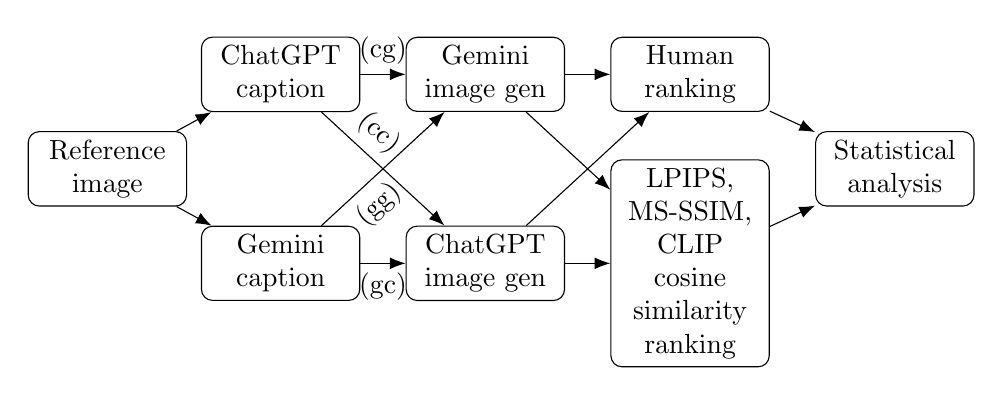
\begin{tikzpicture}[
      x=1mm, y=1mm,
      node/.style={draw, rounded corners, align=center, inner sep=3pt, text width=18mm, minimum height=8mm},
      arrow/.style={-{Latex[length=2mm]}, line width=0.4pt}
    ]
    \node[node] (ref) at (0,0) {Reference\\image};
    \node[node] (cap_cgpt) at (22,12) {ChatGPT\\caption};
    \node[node] (cap_gem) at (22,-12) {Gemini\\caption};
    \node[node] (gen_cgpt) at (48,-12) {ChatGPT\\image gen};
    \node[node] (gen_gem) at (48,12) {Gemini\\image gen};
    \node[node] (rank_h) at (74,12) {Human\\ranking};
    \node[node] (rank_m) at (74,-12) {LPIPS, MS-SSIM, CLIP cosine similarity\\ranking};
    \node[node] (stats) at (100,0) {Statistical\\analysis};

    \draw[arrow] (ref) -- (cap_cgpt); 
    \draw[arrow] (ref) -- (cap_gem);

   % captions -> generators (label variants where they are defined)
\draw[arrow] (cap_cgpt) -- node[midway, sloped, above, xshift=-10pt] {(cc)} (gen_cgpt);
\draw[arrow] (cap_cgpt) -- node[midway, above] {(cg)} (gen_gem);
\draw[arrow] (cap_gem)  -- node[midway, below] {(gc)} (gen_cgpt);
\draw[arrow] (cap_gem)  -- node[midway, sloped, below, xshift= -10pt] {(gg)} (gen_gem);

    \draw[arrow] (gen_cgpt) -- (rank_h);
    \draw[arrow] (gen_cgpt) -- (rank_m);
    \draw[arrow] (gen_gem) -- (rank_h);
    \draw[arrow] (gen_gem) -- (rank_m);

    \draw[arrow] (rank_h) -- (stats);
    \draw[arrow] (rank_m) -- (stats);
  \end{tikzpicture}
  }
  \caption{Experimental workflow applied to the collected reference images: captioning, image generation, ranking, and statistical analysis.}
  \label{fig:workflow}
\end{figure}
\subsection{Image Variants}
Each of the 15 images has a reference version and four model-generated variants (gg)--(cc). Variants differ in composition and style but share the same prompt intent. Table~\ref{tab:variant_mapping} shows the mapping from letters to generator and caption source.
Reference images were collected specifically for this study to minimize the chance that either model encountered them during pretraining (although it is not possible to know whether similar images were in the pretraining data, especially for generic scenes like landscapes and everyday objects). The small bespoke set spans natural elements (landscapes, trees, sky, northern lights), embedded text (for instance, on a traffic sign), everyday objects (flags, food, electronics, games), people, and drawings ensuring diversity in content types that stress both compositional and semantic alignment. Prompts used for captioning and generation are neutral ("describe the image" for captioning; "generate an image based on the following description" for generation).
\begin{table}[!h]
  \centering
  \caption{Mapping from letters (gg)--(cc) to generator and caption source.}
  \label{tab:variant_mapping}
  \begin{tabular}{@{}lcc@{}}
    \toprule
     & Caption: Gemini & Caption: ChatGPT \\
    \midrule
    Generator: Gemini & (gg) & (cg) \\
    Generator: ChatGPT/DALL--E & (gc) & (cc) \\
    \bottomrule
  \end{tabular}
\end{table} 

\subsection{Human Evaluation}
Ten raters (balanced male/female) ranked the four variants for every image. Raters were recruited among students and were blind to model identities. Inter-rater agreement is summarized with Kendall's W per image and averaged. Raters saw all four variants side-by-side on a laptop screen (along with the reference image) and selected a strict ordering after brief instructions about prioritizing semantic fidelity. No time limit was imposed. %Position of variants was fixed.% 
Per-image, per-rater randomization of positions is applied to reduce potential positional bias.
Participants gave informed consent; no personal or identifying data was collected.

\subsection{Automatic Metrics}
LPIPS (AlexNet backbone), MS-SSIM, and CLIP cosine similarity (ViT-B/32) are computed. Images are resized to match references for perceptual metrics. Per-variant means and per-image ``winners'' (best score per metric) are reported.

\subsection{Evaluation Protocol}
For each image, raters view the four candidates simultaneously and rank them 1--4. Top-1 rates (fraction of times a variant is ranked first) are aggregated and Kendall's W is computed to quantify agreement. For automatic metrics, image sizes are aligned to the reference, scores are computed, and variants are ranked per metric and image. Correlations are computed between human mean ranks and metric-induced ranks (scores converted to ranks per image), not between raw scores. 
Bootstrap confidence intervals and Wilcoxon signed-rank tests in Section~\ref{sec:corr_analysis} operate on the 15 per-image Spearman coefficients per metric, treating images as
independent instances of the task.

\section{Results}
\label{sec:results}
\subsection{Human Preferences}
Top-1 rates are: (gg) (44\%), (cg) (22\%), (gc) (13.3\%), (cc) (20.7\%). Inter-rater agreement across all images averages $\bar{W}=0.40$ (Table~\ref{tab:kendall_w}), commonly interpreted as moderate agreement; this loosely upper-bounds how tightly any automatic metric can correlate with the human rankings. Image-level $W$ ranges from low agreement to near-consensus, suggesting image-dependent ambiguity. Fig.~\ref{fig:human_heatmap} summarizes placement percentages across all raters.
Given the mapping, raters most often preferred Gemini-generated images prompted by Gemini captions (gg), followed by Gemini with ChatGPT captions (cg), and least often ChatGPT-generated images conditioned on Gemini captions (gc). The ChatGPT stack with ChatGPT captions (cc) lands between (cg) and (gc), suggesting both the generator and caption source influence perceived quality. The preference table (Table~\ref{tab:pref_table}) shows (gg) outranking (cg) in 63\% of all comparisons, while (gc) vs. (cc) is nearly balanced (47\% vs. 53\%), indicating stronger intra-model consistency for Gemini than for ChatGPT. The mean rank-difference heatmap (Fig.~\ref{fig:mean_rank_diff}) echoes this: the gg--cg row is consistently negative (mean $-0.53$ ranks), whereas gc--cc hovers near zero (mean $0.05$), with several images flipping order.
\begin{figure}[htb]
  \centering
  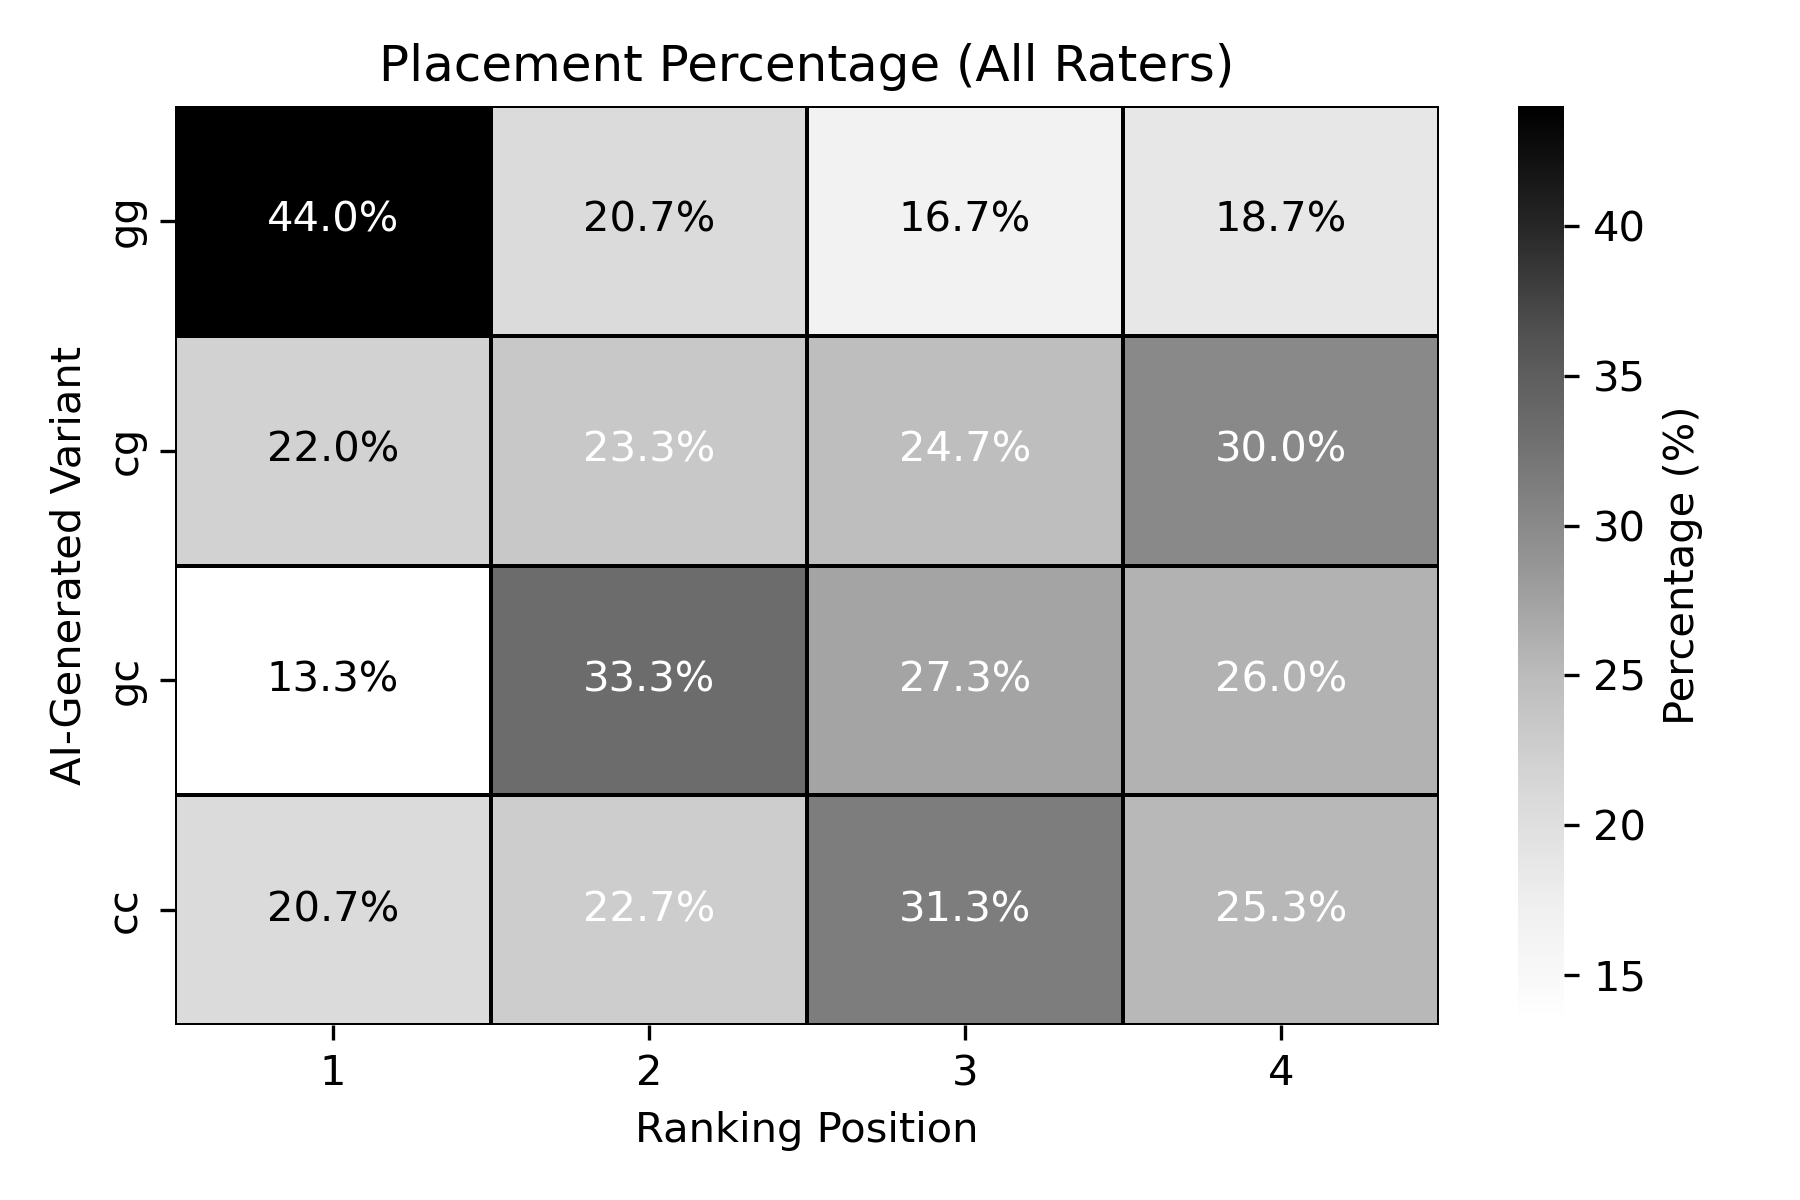
\includegraphics[width=0.9\columnwidth]{../01_basic/analysis/human_preferences_report/overall.png}
  \caption{Human placement percentages across all raters. Variant (gg) is most often ranked first.}
  \label{fig:human_heatmap}
\end{figure}
\begin{figure}[htb]
  \centering
  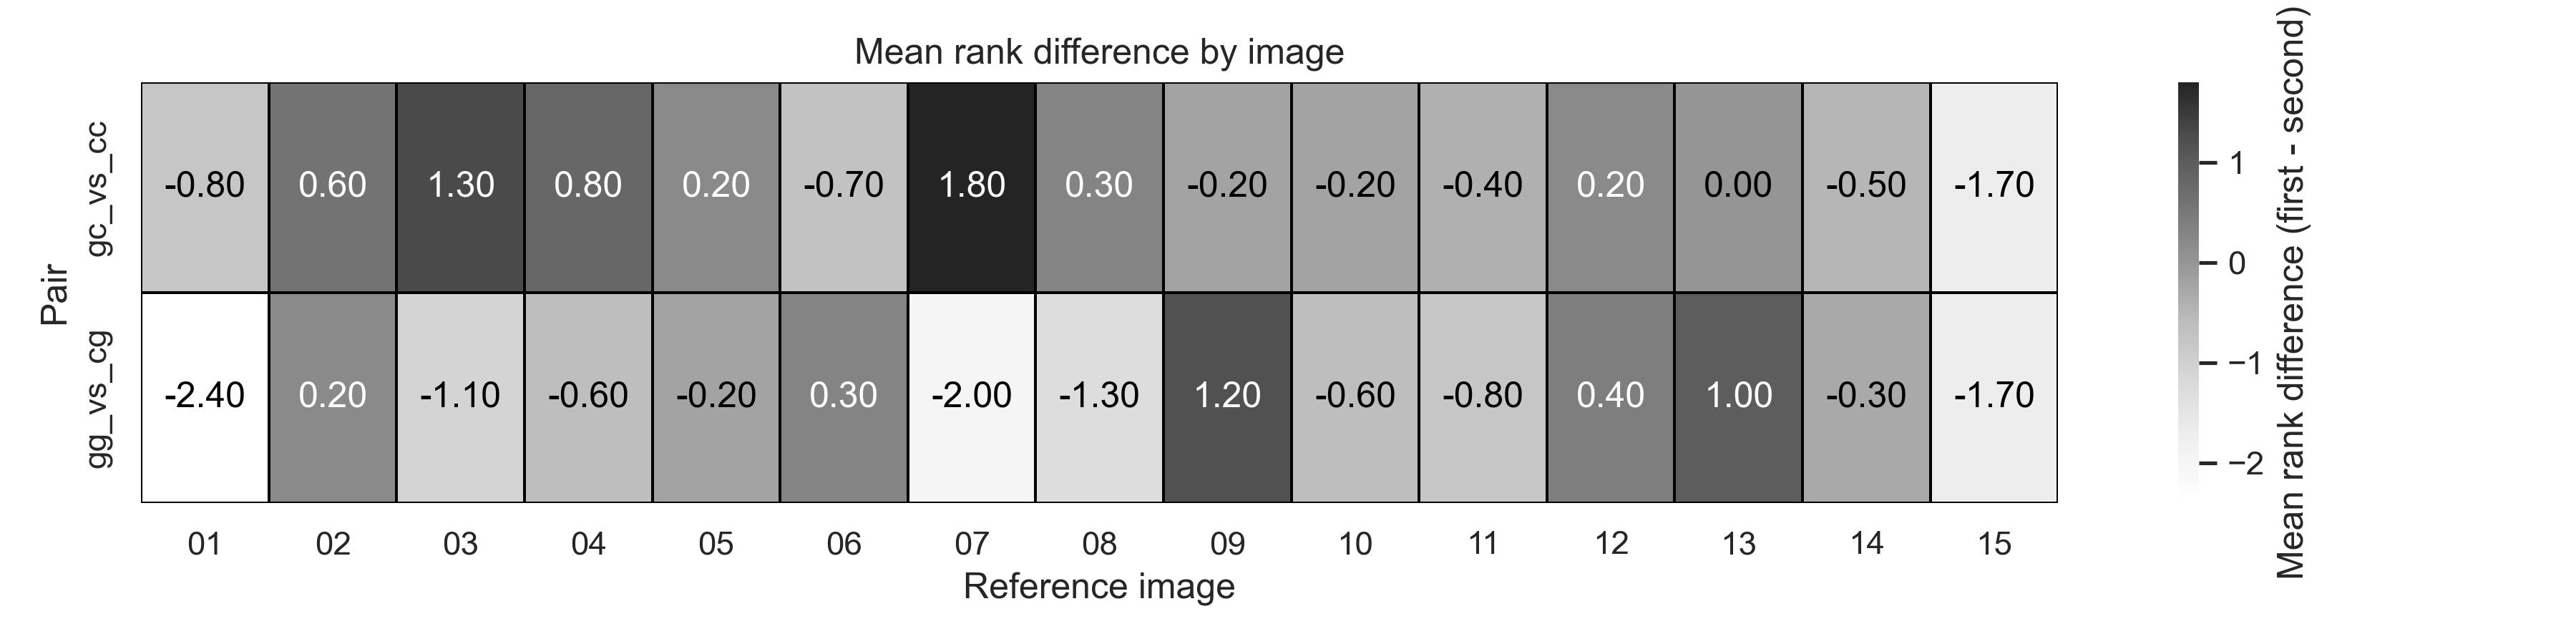
\includegraphics[width=0.9\columnwidth]{../01_basic/analysis/pair_consistency_report/mean_rank_difference_heatmap.png}
  \caption{Mean rank difference (first--second) per image for pairs (gg, cg) and (gc, cc). Negative values mean the first variant is ranked higher.}
  \label{fig:mean_rank_diff}
\end{figure}
\begin{table}[htb]
  \centering
  \caption{Share of comparisons favoring each ordering within the two pairs (percent within pair).}
  \label{tab:pref_table}
  {\scriptsize\setlength{\tabcolsep}{4pt}\renewcommand{\arraystretch}{0.9}%
  \begin{tabular}{@{}lcccc@{}}
    \toprule
    Pair & $gg>cg$ & $cg>gg$ & $gc>cc$ & $cc>gc$ \\
    \midrule
    Percentage & 62.7 & 37.3 & 47.3 & 52.7 \\
    \bottomrule
  \end{tabular}}
\end{table}
\begin{table}[htb]
  \centering
  \caption{Per-image inter-rater agreement (Kendall's $W$); mean $\bar{W}=0.40$.}
  \label{tab:kendall_w}
  {\scriptsize\setlength{\tabcolsep}{2pt}\renewcommand{\arraystretch}{0.9}%
  \resizebox{\columnwidth}{!}{%
  \begin{tabular}{@{}ccccccccccccccc@{}}
    \toprule
    01 & 02 & 03 & 04 & 05 & 06 & 07 & 08 & 09 & 10 & 11 & 12 & 13 & 14 & 15 \\
    \midrule
    0.712 & 0.072 & 0.388 & 0.300 & 0.016 & 0.396 & 0.924 & 0.628 & 0.348 & 0.552 & 0.080 & 0.028 & 0.492 & 0.484 & 0.580 \\
    \bottomrule
  \end{tabular}}}
\end{table}
 
\subsection{Metric Outcomes}
No single metric matches the human-favored variant. Visual inspection confirms that LPIPS and MS-SSIM can reward higher-frequency detail even when humans prefer semantic fidelity, while CLIP occasionally overweights textual alignment. Mean metric scores per variant (lower LPIPS is better; higher MS-SSIM/CLIP is better) are reported in Table~\ref{tab:metric_means}, while Fig.~\ref{fig:metric_winners} shows how often each variant wins per metric. When counting per-image wins (global percentage over all rows), LPIPS favors (gg) (11.7\%) while CLIP favors (gg) (10.0\%) and (cc) (8.3\%); MS-SSIM splits wins across (cg)--(cc) (8.3\% each) with minimal wins for (gg) (1.7\%).
    LPIPS and CLIP lean toward the Gemini-generated images prompted by Gemini captions variant (gg), whereas MS-SSIM spreads wins across Gemini-generated images prompted by ChatGPT captions (cg) and ChatGPT-generated images prompted by ChatGPT captions (cc), indicating that neither Gemini nor ChatGPT pipelines dominate across perceptual criteria. The spread reinforces that off-the-shelf metrics disagree on whether Gemini-generated or ChatGPT-generated images better match references, even when fed the same caption source.
    Fig.~\ref{fig:human_auto_bars} contrasts human top-1 rates with global metric win percentages to highlight where automatic selection diverges from human preference.
    Across metrics, the mean scores in Table~\ref{tab:metric_means} lie in a narrow band, implying that automatic measures view the variants as roughly similar, whereas human preferences are more polarized toward variant (gg), underscoring a gap between numerical similarity and subjective choice.

\begin{table}[b!]
  \centering
  \caption{Mean automatic scores per variant (lower LPIPS is better; higher MS-SSIM/CLIP is better).}
  \label{tab:metric_means}
  {\scriptsize\setlength{\tabcolsep}{4pt}\renewcommand{\arraystretch}{0.9}%
  \begin{tabular}{@{}lccc@{}}
    \toprule
    Variant & LPIPS & MS-SSIM & CLIP cosine \\
    \midrule
    (gg) & 0.743 & 0.399 & 0.788 \\
    (cg) & 0.764 & 0.406 & 0.773 \\
    (gc) & 0.755 & 0.458 & 0.786 \\
    (cc) & 0.764 & 0.443 & 0.790 \\
    \bottomrule
  \end{tabular}}
\end{table}
\begin{figure}[htb]
  \centering
  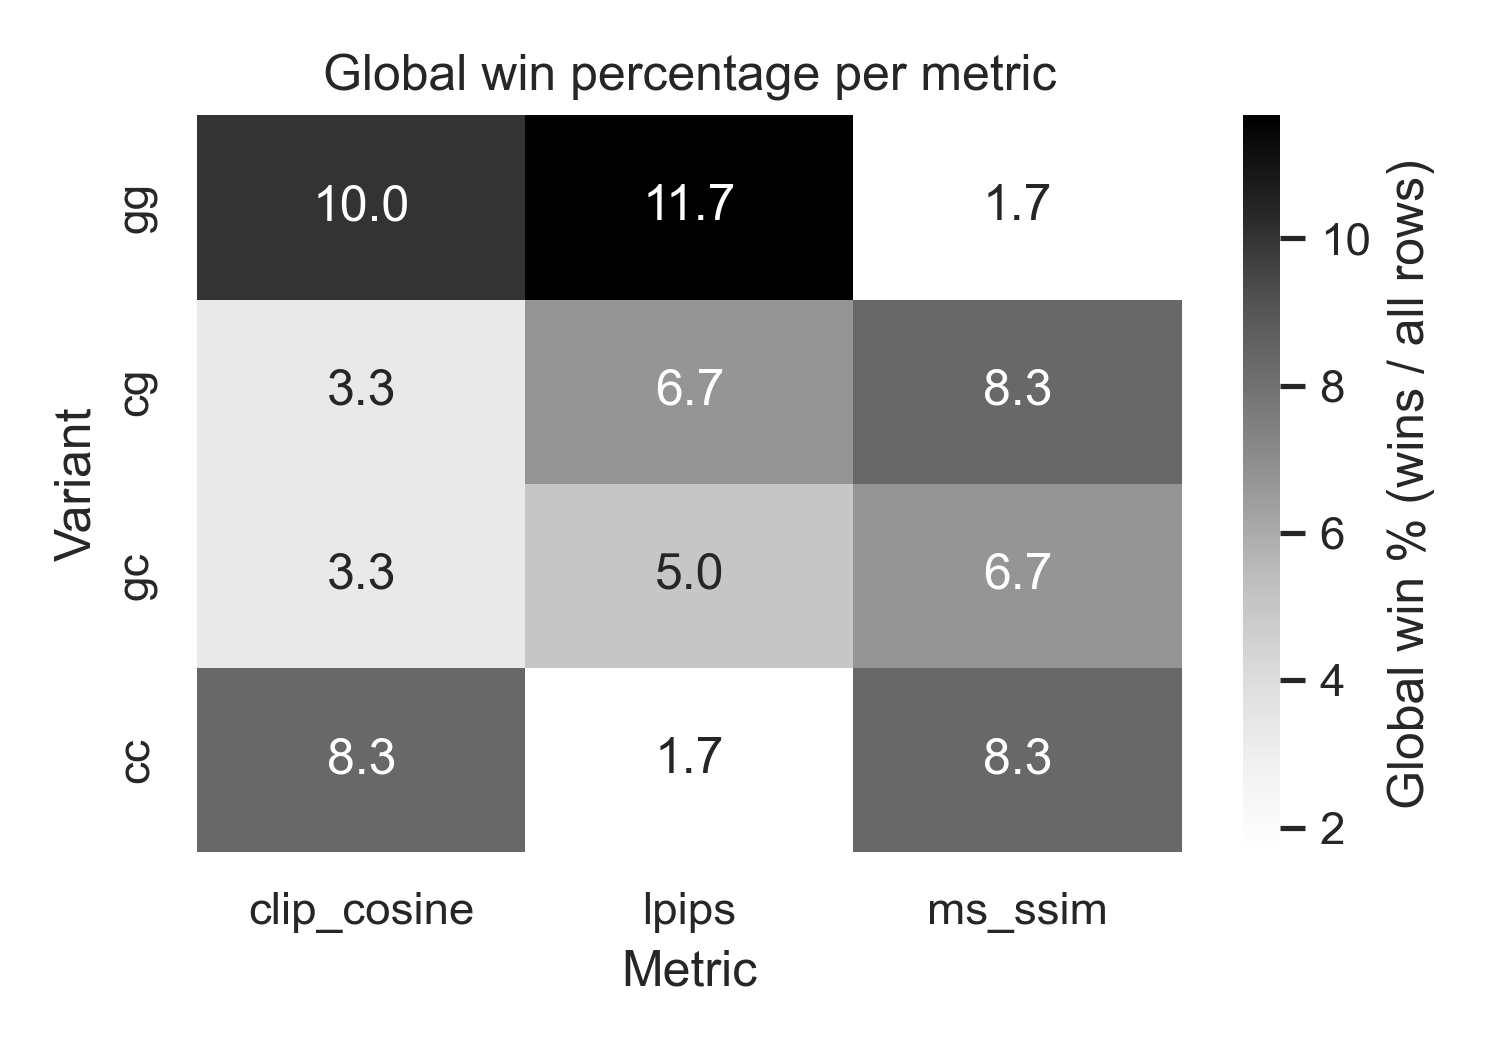
\includegraphics[width=0.9\columnwidth]{../01_basic/analysis/automatic_measures_report/metric_winners_heatmap.png}
  \caption{Global percentage of per-image wins by variant and metric.}
  \label{fig:metric_winners}
\end{figure}
\begin{figure}[htb]
  \centering
  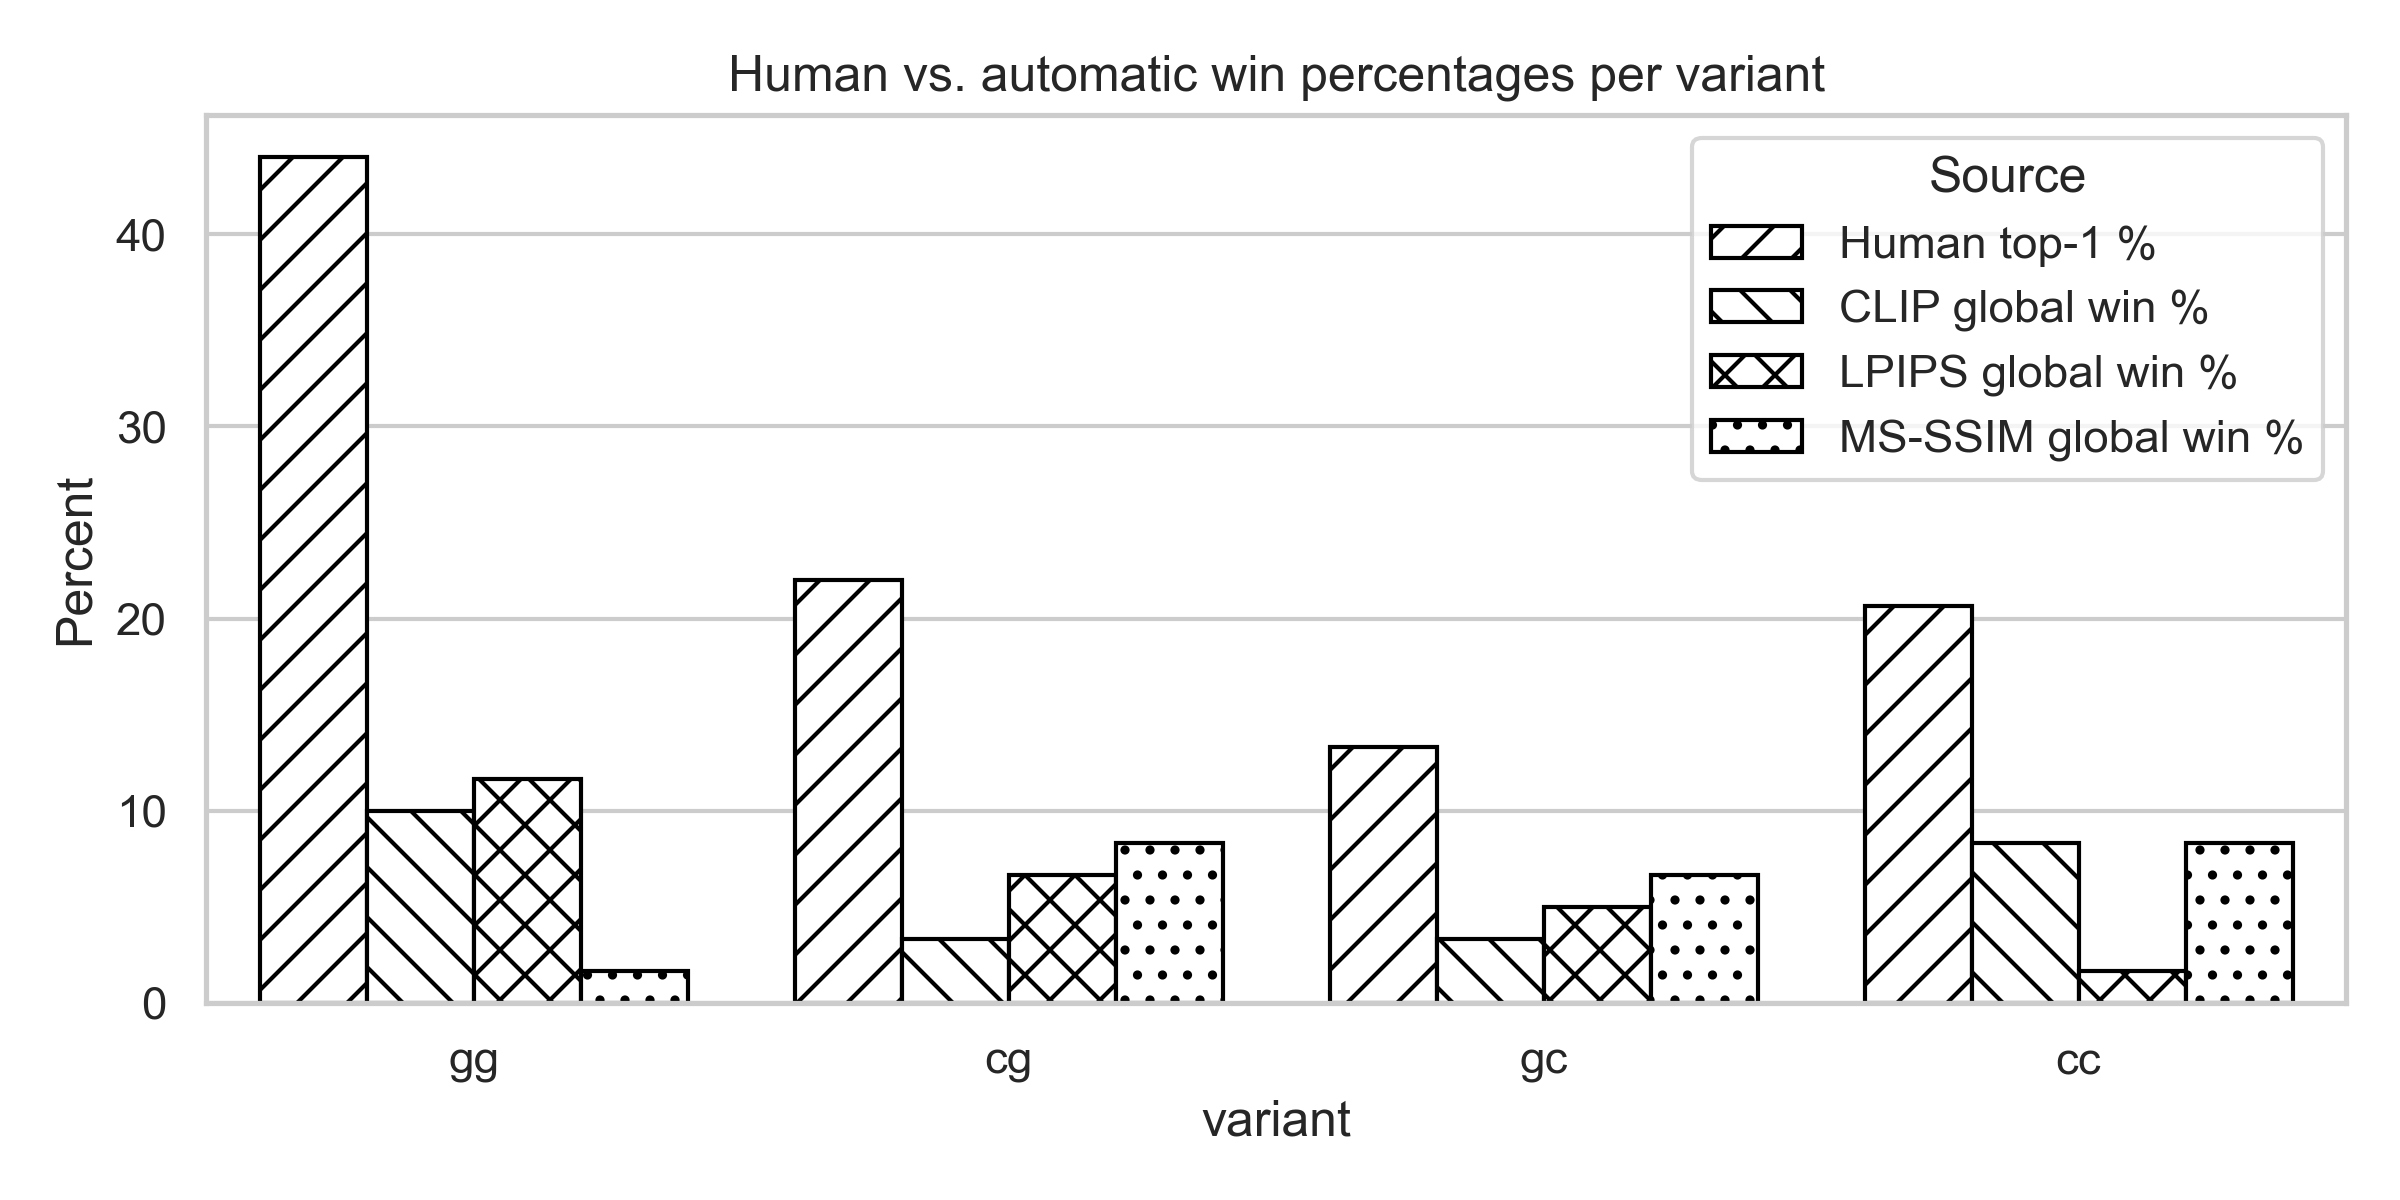
\includegraphics[width=0.9\columnwidth]{../01_basic/analysis/automatic_measures_report/human_vs_automatic_variants.png}
  \caption{Human top-1 rates compared to automatic global win percentages per variant.}
  \label{fig:human_auto_bars}
\end{figure}

%\subsection{Rank Distributions}
%Beyond single winners, the typical rank positions of each variant are examined when ordered by a metric. LPIPS places variant (gg) first most often but also pushes it to lower ranks in some cases. MS-SSIM distributes ranks more evenly, while CLIP concentrates wins on (gg) and (cc). These distributions echo the weak correlations with human preferences: no metric consistently mirrors the human ordering.

\subsection{Correlation Analysis}
\label{sec:corr_analysis}

Table~\ref{tab:corr} reports the mean correlation between human mean ranks and each metric over 15 images. CLIP has the highest mean Spearman (0.36); all bootstrap CIs include zero, but CLIP's interval is shifted upward (0.36 [$-0.02$, 0.67]) relative to LPIPS (0.11 [$-0.25$, 0.46]) and MS-SSIM (0.06 [$-0.29$, 0.40]; Fig.~\ref{fig:spearman_ci}). This is consistent with a modest positive relationship for CLIP but a sample too small to be certain, while LPIPS and MS-SSIM remain fully compatible with no real correlation. A one-sided (directional) Wilcoxon signed-rank test on per-image Spearman values finds CLIP greater than LPIPS ($p{=}0.13$) and greater than MS-SSIM ($p{=}0.07$), indicating only weak evidence that CLIP outperforms the other metrics in this small-$N$ setting. Some images exhibit negative or near-zero correlation, indicating cases where metrics are anti-aligned with human preference.

\begin{figure}[!h]
  \centering
  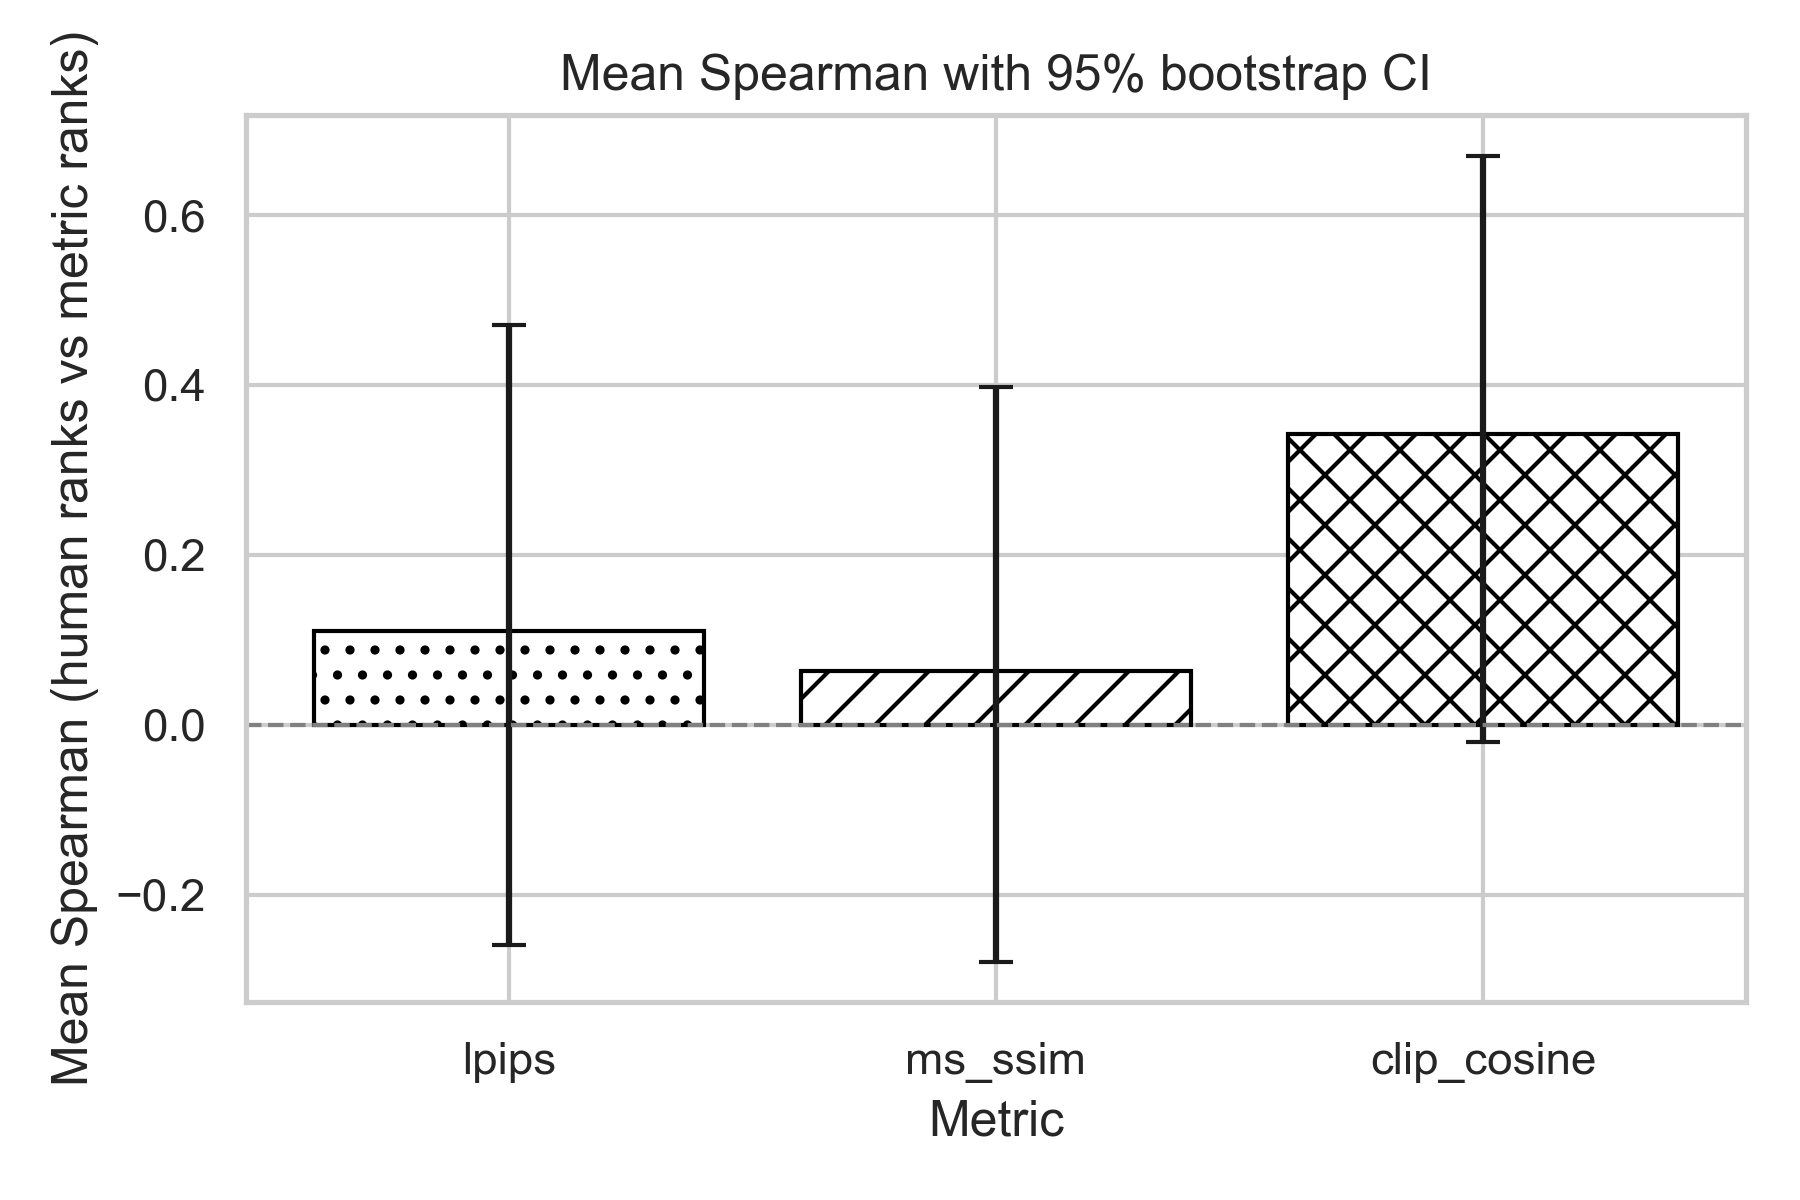
\includegraphics[width=0.8\columnwidth]{../01_basic/analysis/correlation_report/spearman_mean_ci.png}
  \caption{Mean Spearman (human mean ranks vs. metric ranks) with 95\% bootstrap CIs.}
  \label{fig:spearman_ci}
\end{figure}

\begin{table}[!h]
  \centering
  \caption{Mean correlations (15 images) between human mean ranks and automatic metrics.}
  \label{tab:corr}
  \scriptsize
{\setlength{\tabcolsep}{1pt}\renewcommand{\arraystretch}{0.75}%
\begin{tabular}{@{}lccc@{}}
    \toprule
    Metric & Kendall & Spearman & Pearson \\
    \midrule
    CLIP cosine & 0.32 & 0.36 & 0.35 \\
    LPIPS & 0.12 & 0.11 & 0.13 \\
    MS-SSIM & 0.01 & 0.06 & 0.10 \\
    \bottomrule
  \end{tabular}}
\end{table}

\section{Discussion}
Humans prefer variant (gg) nearly twice as often as (cg) and three times as often as (gc), yet automatic metrics do not unanimously select (gg). CLIP tracks human rankings better than LPIPS or MS-SSIM on average, although this advantage is only weakly supported statistically in this small sample (Wilcoxon $p>0.05$), and substantial disagreement remains. Moderate inter-rater agreement ($\bar{W}=0.40$) further limits how strongly any metric can align, suggesting that image difficulty and subjective taste both contribute noise. Since both $\bar{W}$ and the metric–human correlations are computed per image and then averaged, each image acts as an independent instance of the task, and disagreement between raters sets an upper bound on how coherent any metric–human relationship can be on this dataset. The inconsistency across metrics underscores the need for either metric ensembling, human-in-the-loop ranking, or task-specific fine-tuning. Expanding rater diversity and scale is future work. Practical guidance: if constrained to a single metric, CLIP is the least misaligned here; otherwise, collect a small human validation set and calibrate a weighted combination.

\subsection{Limitations}
The study covers only 15 images and four variants per image, limiting statistical power and diversity. Rater demographics are narrow (ten participants), so subgroup analysis is indicative only. All metrics are used off-the-shelf; better alignment may be achievable with fine-tuned or task-specific preference models. Images are evaluated at a single resolution and device configuration; %variants were shown in fixed positions, which may introduce mild positional bias, and% 
different scales or hardware could modestly shift scores.

\subsection{Practical Implications}
For small-batch creative workflows where a designer must pick one of several candidates, these pilot results (15 images, $\bar{W}=0.40$) suggest that a semantic signal such as CLIP may be a safer default than purely perceptual scores, but this is a hypothesis rather than a validated prescription. A pragmatic design idea is to pair one semantic metric with a quick human pass, or to learn metric weights on a small, task-specific human calibration set; both would need targeted testing. In automated pipelines, exposing multiple candidates to end users may be preferable to auto-selecting a ``best'' image based solely on any single off-the-shelf metric.

\subsection{Future Directions}
Expanding the image set and rater pool would allow finer-grained subgroup analysis and statistical testing.
%Per-image, per-rater randomization of positions could reduce potential positional bias.%
Prompt engineering is another avenue: future experiments can explicitly provide models with information about the target audience and task purpose when generating captions or images. For captioning, the audience cue can specify whether the consumer is the same model that will later generate images or a different AI model. For generation, prompts can state whether the output is destined for human ranking or an automatic tool, enabling evaluation of how audience- and purpose-aware instructions affect alignment.

\section{Conclusion}
This study had two research questions: how consistent are ChatGPT and Gemini in aligning descriptions and generations, both within the same model and across different models (RQ1), and how well do LPIPS, MS-SSIM, and CLIP cosine similarity align with human judgments (RQ2). The main findings are:
\begin{enumerate}
  \item[RQ1] Raters favored Gemini-generated images prompted by Gemini captions (variant (gg)), with lower preference for ChatGPT-generated images; intra-model consistency is stronger than inter-model consistency, since each model paired with its own captions ((gg) and (cc)) is ranked first more often than when using the other model's captions ((cg) and (gc)). Table~\ref{tab:pref_table} and Fig.~\ref{fig:mean_rank_diff} highlight this: (gg) beats (cg) in 63\% of pairwise comparisons and is, on average, half a rank better, while (gc) vs. (cc) is nearly split with small mean differences, highlighting how ChatGPT shows weaker dependence on caption source than Gemini in this pilot setting.
  \item[RQ2] CLIP shows the strongest (yet modest) alignment with human rankings, while LPIPS and MS-SSIM correlate weakly, so no single automatic metric adequately proxies human judgment.
\end{enumerate}
All code for metric computation and analysis, together with anonymized images, captions,
and rankings, is available at https://github.com/SaverioNapolitano/qrd.
\begin{thebibliography}{00}
\bibitem{lpips} R. Zhang \emph{et al.}, ``The Unreasonable Effectiveness of Deep Features as a Perceptual Metric,'' in \emph{CVPR}, 2018.
\bibitem{clip} A. Radford \emph{et al.}, ``Learning Transferable Visual Models From Natural Language Supervision,'' in \emph{ICML}, 2021.
\bibitem{ssim} Z. Wang \emph{et al.}, ``Image quality assessment: From error visibility to structural similarity,'' \emph{IEEE TIP}, 2004.
\bibitem{msssim} Z. Wang \emph{et al.}, ``Multi-scale Structural Similarity for Image Quality Assessment,'' in \emph{Asilomar}, 2003.
\bibitem{clipscoreshuster} S. Huster \emph{et al.}, ``CLIPScore: A reference-free evaluation metric for image captioning,'' \emph{EMNLP}, 2021.
\bibitem{fid} M. Heusel \emph{et al.}, ``GANs Trained by a Two Time-Scale Update Rule Converge to a Local Nash Equilibrium,'' in \emph{NeurIPS}, 2017.
\bibitem{wu2023survey} J. Wu \emph{et al.}, ``Multimodal Large Language Models: A Survey,'' in \emph{IEEE Big Data}, 2023.
\bibitem{yu2025survey} T. Yu \emph{et al.}, ``Aligning Multimodal LLM with Human Preference: A Survey,'' \emph{arXiv:2503.14504}, 2025.
\bibitem{tang2024clipagiqa} Z. Tang \emph{et al.}, ``CLIP-AGIQA: Boosting the Performance of AI-Generated Image Quality Assessment with CLIP,'' in \emph{ICPR}, 2024.
\bibitem{liu2023geval} Y. Liu \emph{et al.}, ``G-Eval: NLG Evaluation Using GPT-4 with Better Human Alignment,'' in \emph{EMNLP}, 2023.
\end{thebibliography}
 
\end{document}
